\documentclass[10pt]{article}
\usepackage[utf8]{inputenc}
\usepackage[italian]{babel}
\usepackage{multicol}
\usepackage[a4paper, total={18cm, 25cm}]{geometry}
\usepackage{array}
\usepackage{graphicx}
\graphicspath{ {./img/} }
\begin{document}
\title{Programmazione d'Interfacce}
\author{Federico Matteoni}
\date{ }
\renewcommand*\contentsname{Indice}

\maketitle
\tableofcontents
\pagebreak
\section{Introduzione}
Appunti del corso di \textbf{Programmazione d'Interfacce} presi a lezione da \textbf{Federico Matteoni}.\\More like \textit{design d'interfacce}.\\\\
Prof.: \textbf{Daniele Mazzei}, mazzei@di.unipi.it\\
\begin{list}{-}{Riferimenti web:}
\item \emph{?}
\end{list}
Esame: compitini/scritto + orale discorsivo dove si discute un software noto.\\Possibile proporre un software personale da presentare all'esame orale, spiegando come si è applicati i rudimenti del corso sul software presentato.\\\\
\begin{list}{-}{Materiale didattico:}
\item \textbf{Google Classroom}, slide presentate a lezione e altro materiale didattico\\Codice \textbf{c14kiy} con le credenziali d'ateneo.\\La suite Google è attivabile a \emph{start.unipi.it/gsuite}\\\textit{Non è autorizzata la divulgazione}
\item La Caffettiera del Masochista, Donald A. Norman\\Eng: The Design of Everyday Things
\item Designing the User Interface, Ben Shneiderman
\item \emph{www.usability.gov}
\item \emph{interaction-design.org}
\end{list}
Ricevimento: Mercoledì 14.30-16, Stanza 366\\

\section{Il Corso}
\textbf{Interface Development in 2020} diventa \textbf{Interface Design in 2020}
\paragraph{Diviso in due parti}
\begin{list}{-}{}
\item \textbf{UX e UI} con introduzione, UI vs UX, HCI, paradigmi, gamification...
\item \textbf{Strumenti per lo sviluppo dell'interfaccia utente} presentati da vari ospiti: Unity, Zerynth, Ubidots, Angular, Amazon Lex, ...
\end{list}

\textbf{Interfaccia} è qualsiasi metodo utilizzato da una persona per \textbf{interagire} con un dispositivo.

\section{Design}
\paragraph{Cos'è il design} Il design è la \textbf{pianificazione o la specifica per la costruzione di un oggetto o sistema} o per l'implementazione di un'attività o processo. Diventa l'esatto opposto della decomposizione del problema in sottopassaggi, cioè del pensiero computazionale. Il design parte dalla base del problema e \textbf{identifica soluzioni per la causa del problema}. Si può avere anche il design di una strategia di implementazione.\\
\quotedblbase \textbf{Bisognerebbe progettare le applicazioni come se fossero persone che ci piacerebbe frequentare}\textquotedblright. Ad esempio Netflix, o il frigorifero.

\subsection{XX Designer}
Discernere tra Graphic Design, User Experience Design (UX Design) e User Interface Design (UI Design).
\paragraph{UX}: come l'utente si sente per interagire e cosa vuole fare. Aspetto più psicologico, guida la UI design in base a statistica fatta su gruppi di utenti. Manda "\textit{l'output}" a chi fa UI e al marketing.\\
\paragraph{UI}: come l'utente interagisce col prodotto (shortcut, sottomenu...)\\
\subsubsection{UX Designer}
Si deve porre il problema di quali approcci usare per risolvere problemi evidenziati da analisi di mercato.\\
\textbf{Chi paga non è detto che sia chi usa il servizio}. Ad esempio Netflix viene pagato da una persona, ma lo stesso account viene usato anche da altre persone (anzi, in particolare \textbf{il 90\% del tempo} chi usa l'account non è chi paga).\\
Uno dei metodi usati per fare UX è quello della \textbf{definizione delle \textbf{personas}} (cioè un archetipo di utente). Una persona può assumere diverse personas.
\paragraph{User Experience} Con User Experience si parla del prodotto e di come si comporta nel mondo reale, che è fatto di \textit{personas}.
\textbf{Non si può progettare \textit{una user experience}, si può progettare \textit{per la user experience}}. La user experience è ciò che fa l'utente, e lo sviluppatore non ha controllo su ciò. L'utente si approccia al software come gli pare.
\subsubsection{UI Designer}
Dalla UX si crea lo \textbf{sketch} dell'interfaccia. Non viene prodotto subito il wireframe ma bisogna partire da altro, ad esempio dai \textbf{casi di studio}. Esistono più casi di studio per ogni personas (casalinga voghera che fa bonifico, casalinga voghera che cambia password, ecc.). Ogni caso di studio è \textbf{specifico per personas}, poiché personas diverse hanno capacità diverse (non conoscere alcuni concetti, non saper fare determinate operazioni...).\\
L'\textbf{UI design è un procedimento diverso dal front-end developing}, quindi possono essere persone separate. Il designer progetta le guideline che istruiscono il developer.\\
Si può dire che la UI design è sottoarea di UX design.\\

\subsection{Front-End Developer}
Esegue il design della UI convertendolo in funzionalità del prodotto.\\

\section{Interfacce Utente}
\paragraph{L'interfaccia utente (UI)} L'UI di un sistema è \textbf{lo spazio dove avviene l'interazione uomo-macchina}: lo schermo, le casse, il mouse e quant'altro.\\
L'obiettivo dell'interfaccia è far si che \textbf{l'utente possa controllare la macchina}, e \textbf{non il contrario}. L'interfaccia può però influenzare il comportamento dell'utente, ad esempio se voglio guidare l'utente in un particolare modo l'interfaccia deve dare un feedback tale da guidare l'utente.\\
L'altro obiettivo dell'interfaccia è \textbf{rendere fruibile \textit{in maniera piacevole} le funzionalità che una macchina eroga} verso l'utente. Il termine \textbf{user-friendly} non può essere omesso: tra un'app facile e piacevole da usare e una solo facile da usare, l'utente medio preferirà sempre la prima.\\
L'interfaccia è strutturata a layer. lo HID (Human Interface Device) è la periferica con cui l'umano interagisce col sistema. Questo server per usare più HID per interagire con diverse applicazioni.\\
HMI (Human Machine Interface) è più astratta rispetto a HCI (Human Computer Interface), quindi in HMI è più teorica la cosa.
\paragraph{Diversi tipi di interfacce} Abbiamo 5 sensi, quindi diverse \textbf{categorie d'interfaccia}: le più comuni sono \textbf{grafiche} e \textbf{tattili} (\textbf{GUI}, Graphical User Interface). Se si aggiunge anche il suono diventano \textbf{MUI} (Multimedia User Interface). Il concetto di GUI è stato coniato in un tempo in cui l'audio era raro. Adesso \textbf{praticamente tutte le interfacce sono MUI}.\\
Esempio di MUI riprogettata in GUI: Facebook. I video partivano in automatico con l'audio attivo, mentre ora sono mutati. Poi sono stati aggiunti i sottotitoli automatici: questo è un esempio di tecnica ideata per le utentze disabili e riusata per poter far fruire il prodotto a quelle personas che in quel momento non possono usufruire dell'audio. \textit{Meglio un sottotitolo sbagliato che niente}.
\paragraph{Categorizzare interfacce} Le CUI (Composite User Interfaces) sono le UI che interagiscono con due o più sensi.
\begin{list}{}{Esistono tre diverse macrocategorie di CUI:}
\item \textbf{Standard}, che utilizzano dispositivi standard come tastiere, mouse e monitor
\item \textbf{Virtuale}, che \textbf{bloccano il mondo reale e creano un mondo virtuale} e tipicamente utilizzano dei caschi VR
\item \textbf{Aumentata}, che \textbf{non blocca il mondo reale e eroga contenuti non completamente digitali}, ma che prendono dalla realtà esterna che circonda l'utente
\end{list}
Le CUI possono anche essere \textbf{classficiate per il numero di sensi} con cui esse interagiscono. Per esempio, lo \textit{Smell-O-Vision} è una CUI standard 3S (3 sensi) con un display, suono e odori. Se si aggiungesse la vibrazione della poltrona, diventerebbe 4S poiché si aggiunge il tatto.\\
Si parla di \textbf{Qualia Interfaces} quando si stimolano tutti i sensi.
\paragraph{Mancata evoluzione} Le UI \textbf{sono le stesse di 10 anni fa}. Bisogna mettere in discussione i paradigmi attuali. L'industria ha convertito l'ambiente fisico della scrivania in ambiente digitale, prendendo ispirazione dall'abitudine dell'utente per rendere più semplice il passaggio. Ora l'utente è abituato, la realtà da cui si prende spunto non esiste più. Bisogna cambiare.

\section{Good and Bad Design}
\textbf{Il buon design non esiste}, poiché si fa design \textit{per} la user experience \textbf{di una determinata personas}.
\begin{list}{}{Le due caratteristiche più importanti su cui misurare il buon design sono:}
\item \textbf{Discoverability}: è la \textbf{capacità innata di un sistema di veicolare i possibili usi e dire come si usa}. Non è detto che una volta che si è capito cosa si può fare si riesca a farlo.\\
Per avere buona discoverability si usa tipicamente la visibilità: un rubinetto con i pomelli bene in vista incrementa la discoverability. Nel software, \textbf{questo lavoro lo fanno i pulsanti}.
\item \textbf{Understanding}: è la \textbf{capacità di comprendere i possibili usi}. Ad esempio: il fornello, è in cucina quindi so che si usa per scaldare ecc., il problema maggiore però è il mapping pomello $\rightarrow$ fornello. Si può risolvere con l'icona del fornello corrispondente, ma non risolve effettivamente il problema. Una soluzione efficacie è disporre fornelli e pomelli in modo che sia evidente la correlazione fra essi.\\
\textbf{Non sottovalutare il costo mentale dell'utente}.
\end{list}
\begin{center}
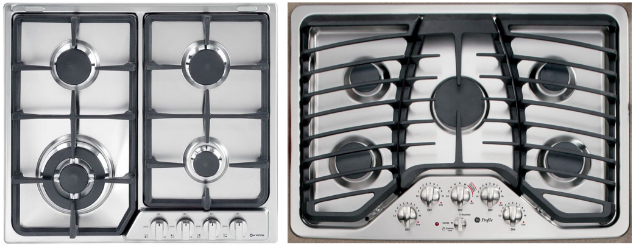
\includegraphics[scale=0.5]{fornelli.png}
\end{center}

\subsubsection{Design of Useful Things}
\paragraph{Il paradosso di TripAdvisor} \quotedblbase \emph{Quando la gente mangia bene, non recensisce. Quando mangia male, recensisce}\textquotedblright.
\paragraph{Sensazioni} Quando le cose vanno bene, si dimenticano subito. Questo perché, in qualche modo, l'uomo pensa che \textbf{le cose vadano bene per definizione}. Quando qualcosa va storto, invece, \textbf{l'amigdala crea un ricordo con un peso molto maggiore}.\\
Il design deve quindi preoccuparsi di come funzionano le cose, come vengono controllate e della natura delle interazioni. Quando la progettazione è fatta bene, crea prodotti piacevoli e brillanti. Quando è fatta male, i prodotti sono inutilizzabili e ciò porta a notevole frustrazione e irritazione.\\
\textbf{Marcatore somatico}: ricordo le esperienze in base alle sensazioni che provavo durante esse. \textbf{Più forte è la sensazione più si cementifica il ricordo}. Ad esempio se faccio un incidente ad una curva, la ricorderò bene per molto tempo. La strada che faccio per andare in vacanza non la ricordo più già al ritorno.\\
\textbf{Con il software si applica lo stesso discorso}. Se non riesco ad usare un programma inizio a provare frustrazione. Gli umani non informatici tengono a ritenere le macchine come superintelligenti, quindi associano alla frustrazione l'incapacità personale: \textbf{se credo di non essere in grado di usare il software non ci riprovo}.\\
Confrontando IA e intelligenza umana, l'IA risulta strettamente limitata a computazione e risoluzione di problemi logici. Al contrario, \textbf{la mente umana non funziona ad algoritmi ma procede per deduzione}. Per lo più generando ipotesi senza fondamento e autoconvincendosene.\\
Le macchine seguono regole semplici: gli algoritmi. Essi non hanno la flessibilità (\textbf{common sense}) tale da assecondare l'utente. Per esempio, se chiedo telecomando per l'aula D2 ma non esiste o non c'è il proiettore, la signora mi corregge in D1 e dà il telecomando corretto. La macchina dice semplicemente che non esiste l'aula D2 o il proiettore in aula D2.\\
\textbf{Le macchine non hanno buonsenso}. La maggiorparte delle regole sotto il software sono note solo agli sviluppatori. Potrebbe andare bene, basta renderle discoverable.\\\\
Bisogna invertire il paradigma attuale: se qualcosa va storto \textbf{è colpa dello sviluppatore} e non dell'utente. \textbf{Il dovere della macchina è essere comprensibile} da parte dell'utente.\\\\\textbf{Bisogna accettare che il comportamento umano è com'è e non come vogliamo che sia.}
\section{Human Centered Design}
\textit{Alla fine di ogni passaggio c'è l'utente}.\\Si tratta di una norma \texttt{ISO 9241-210:2010(E)}.
\paragraph{Un approccio} Lo HCD è un \textbf{approccio di design} specificamente orientato allo sviluppo di sistemi interattivi con l'\textbf{obiettivo di fare sistemi utili, altamente usabili e che si focalizzino sull'utente}. Il metodo è orientato \textbf{all'efficienza ed all'efficacia}, per aumentare la soddisfazione dell'utente ed evitare il più possibile gli effetti negativi.\\
\paragraph{Prima l'utente, poi le features} Lo HCD mette \textbf{i bisogni, comportamenti e capacità umane prima di tutto, e progetta in funzione di esse}.\\
Significa che se devo risolvere un problema, non mi interessa risolverlo completamente ma raggiungere il miglior risultato che posso far ottenere all'utente che usa il mio software. Se il \textit{70\% degli utenti raggiungono il proprio scopo} col nostro software, allora esso ha un'\textit{efficacia del 70\%}. Posso puntare ad un'efficienza maggiore magari risolvendo una parte minore del problema.\\
\textit{Less is more.} Meglio una feature in meno che una in più. Ogni volta che aggiungi una feature devi dimostrare perché e a cosa serve, perché tale feature va: spiegata, testata, mantenuta oggi e domani (\textbf{backward compatibility}).\\\\
Il problema principale delle UI è un \textbf{problema di comunicazione} in particolare dalla macchina verso la persona. Una buona interfaccia sa comunicare con l'utente.\\
Progettare interfacce che funzionano egregiamente fintanto che le cose vanno bene è relativamente facile, ma \textbf{la comunicazione è ancora più importante quando le cose non vanno bene}: entrano in gioco le \textbf{strategie di mitigazione dell'errore}. Si focalizza l'interazione soprattutto nel \textbf{comunicare ciò che è andato storto}, in quel momento devo aiutare l'utente frustrato a risolvere il problema perché se lo aiuto a risolvere il problema da solo proverà una sensazione positiva di successo per aver capito cosa non funzionava. Ciò \textbf{crea empatia col sistema}.\\Quindi bisogna \textbf{evitare la frustrazione}, e \textbf{aiutare a risolvere} quando insorge un problema.
\paragraph{Capire l'utente} Lo HCD è una filosofia di design che parte dalla \textbf{comprensione delle persone e dei bisogni} che si intende soddisfare. Spesso gli utenti non si rendono conto dei loro effettivi bisogni e nemmeno delle difficoltà che incontrano.\\
Per capire l'utente la tecnica più utilizzata è l'osservazione. Non è detto sia sempre possibile. Versioni alpha e beta non servono solo debuggare il software, ma servono anche a capire ciò che fanno gli utenti. Diventa utile avere statistiche sull'utilizzo effettivo del sistema: quanti click su un determinato pulsante, quante volte una determinata procedura finisce e così via.\\
\textbf{Le specifiche dello HCD}, quindi, \textbf{nascono dalle persone} e per questo \textbf{non si possono scrivere}. Quindi risulta essere un paradigma che si sposa bene con la computer science perché va avanti per iterazioni: si esegue una specifica ad alto livello, ne implemento una parte, la testo sull'utente reale e tramite il feedback modifico la parte implementata e ri-testo. Quando ritengo buono ciò che ho prodotto lo congelo, e passo ad implementare un'altra parte dell'interfaccia.\\
\begin{multicols}{2}
\begin{tabular}{ c | m{10em} }
\multicolumn{2}{c}{ \textbf{Il ruolo dello HCD nel design} }\\
\hline
Experience design & Area di focus\\
\hline
Industrial design & Area di focus\\
\hline
Interaction design & Area di focus\\
\hline
Human Centered Design & Il processo che assicura che la progettazione incontra i bisogni e le capacità degli utenti che useranno il sistema
\end{tabular}
\columnbreak

Possiamo progettare per esperienza utente, il design industriale e progettare per l'interazione. lo HCD non è area di focus del processo di design ma è metodo.\\Utilizzo l' HCD per progettare tutto il resto.
\end{multicols}
\section{Design Thinking vs HCD}
Insieme al termine Human Centered Desing, spesso si può vedere il termine \textbf{Design Thinking}. I termini vengono da due scuole di pensiero molto forti ma con visioni diverse.
\paragraph{Cos'è il Design Thinking} Il \textbf{Design Thinking} segue il filone Stanford, dove è nato: è un \textbf{processo di design} con cui \textbf{progettare nuovi prodotti} che verranno \textbf{effettivamente adottati dalle persone}. Come processo è più vicino alla disruptive innovation che all'antropocentricità.\\
\textbf{Metodo}, strumento per sviluppare prodotti innovativi. Per sviluppare qualsiasi modello di business orientato all'essere profittevole.\\
Si suddivide in 5 fasi iterative.
\subparagraph{Empathize} \textbf{Studiare} il proprio pubblico. Progettare il prodotto in modo che stabilisca un collegamento empatico con l'utente.
\subparagraph{Define} Delineare meglio le \textbf{domande chiave}, cioè quali sono i bisogni a cui assolvere.
\subparagraph{Ideate} \textbf{Brainstorming}, creare soluzioni.
\subparagraph{Prototype} \textbf{Costruire} una o più idee.
\subparagraph{Test} \textbf{Testare} le idee e \textbf{ricevere feeback}.
\paragraph{HCD e DT} Lo HCD è un mindset che viene sovrapposto al design thinking, il quale è orientato a garantire che le idee siano rilevanti e beneficiali, sul lungo termine, per le persone obiettivo.\\
Lo HCD quindi viene sovrapposto all design thinking: identificato il modello di business, uso lo HCD per sincerarmi che la famiglia di soluzioni identificate venga "pulita", attraverso un processo che \textbf{garantisce l'usabilità da parte di soggetti umani}.\\
\begin{center}
\begin{tabular}{ m{8cm} | m{8cm} }
\textbf{Design Thinking} & \textbf{Human Centered Design}\\
\hline
Processo iterativo a 5 fasi che porta all'effettivo sviluppo di prodotti/soluzioni che verranno adottate dall'utente finale desiderato & Mentalità e strumento da applicare insieme al Design Thinking che crea un impatto a lungo termine positivo, per gli utenti della soluzione\\
\hline
\end{tabular}
\end{center}
Quando l'ispirazione (divergente: produrre idee) cala, si passa all'ideazione (convergente: unire le idee simili, scartare idee ridondanti...).
\section{Principi Fondamentali dell'Interazione}
\paragraph{Life is made of experiences} Bravi designer producono \textbf{esperienze} piacevoli. L'esperienza è molto importante, perché determina quanto bene gli utenti si ricorderanno l'interazione.
\paragraph{Cognizione ed Emozione} Quando la tecnologia si comporta in maniera inaspettata, proviamo confusione, frustrazione e rabbia: \textbf{emozioni negative}. Quando invece comprendiamo il comportamento della tecnologia, abbiamo una sensazione di controllo, bravura e persino orgoglio: \textbf{emozioni positive}. \textbf{Cognizione ed emozione sono profondamente legate}. Se non metto l'utente in un \textbf{mood positivo} farà più fatica ad apprendere l'interfaccia. Più mi arrabbio meno sono predisposto a comprendere e riutilizzare il prodotto.
\subsection{Sei Fondamenti} La \textbf{Discoverability}, cioè il grado di facilità con cui un utente \textbf{scopre come funzione l'interfaccia}, è il risultato della corretta applicazione di sei principi psicologici.
\subsubsection{Affordance}
Il termine \textbf{affordance} si riferisce alla \textbf{relazione tra un oggetto fisico e una persona}: precisamente la relazione tra \textbf{le proprietà di un oggetto e le capacità dell'utente che determinano i possibili utilizzi dell'oggetto}.\\
\textbf{Questa proprietà determina il modo con cui l'oggetto può essere usato.}\\
\emph{"Cosa posso fare sull'interfaccia"}.
\paragraph{Esempi} \textbf{Un pulsante di una UI}, da premere con uno HID che sia il dito o il mouse, \textbf{è un oggetto fisico}. Il pulsante \textit{afforda} (\textbf{consente}) l'essere premuto.\\
Una sedia \textit{afforda} il sostenere, quindi \textit{afforda} di sedercisi.\\
Un potenziometro \textit{afforda} l'essere ruotato.
\paragraph{Tipi di affordance} Ci sono affordance \textbf{innate nel cervello}, \textbf{forme} che il sistema visivo e il cervello interpretano automaticamente.\\
L'affordance è una \textbf{proprietà scaturita da una relazione con un particolare soggetto} (quindi è peculiarità della relazione). Ad esempio, una poltrona \textit{afforda} il sostenere per quasi tutti, ma lo spostamento non è detto sia \textit{affordato} per tutti (per esempio una persona debole non può spostare la poltrona).\\
\textbf{Anti-affordance}: prevenzione dell'interazione. Ad esempio degli spunzoni per evitare che piccioni si posino su un cornicione, \textbf{prevengono l'\textit{affordance} che il cornicione ha verso i piccioni di sedersi}.\\
Affordance e anti-affordance \textbf{devono essere discoverable e percievable}. Questo fatto non è scontato: il vetro \textit{afforda} l'essere attraversato dalla luce e non \textit{afforda} l'essere attraversato dalla materia, ma si può non vedere e \textbf{percepire una falsa \textit{affordance}} di passarci attraverso... e ci batto.\\
Un altro esempio: anche a schermo spento, lo smartphone ha comunque l'\textit{affordance} di essere premuto.\\\\
Assolutamente sbagliato dire che "metto un \textit{affordance}". Posso dire che "metto un significante", ma solo se ho un'\textit{affordance}. I tre pallini per il tasto menu sono un \textbf{significante}.
\subsubsection{Signifiers}
I designer hanno problemi pratici: devono sapere come progettare le cose per renderle understandable. Un significante è un \textbf{modo per indicare dove applicare un determinato \textit{affordance} per ottenere un risultato}
\paragraph{Esempi} Un box quadrato in una GUI (un pulsante) è un \textbf{significante}: se applichi l'\textit{affordance} "tocco" qua ottieni un determinato risultato.\\
L'\textit{affordance} del touch, lo slide, il pinch... esiste su tutto lo schermo. L'\textit{affordance} dice \textbf{cosa} posso fare, il significante dice \textbf{dove} fare l'azione.\\
A volte \textbf{i significanti sono indispensabili} perché la maggiorparte delle \textit{affordance} sono invisibili. I significanti servono per fare capire le \textit{affordance} che non si vedono. Per esempio, le porte scorrevoli: se non vedo i cardini, quando vedo la maniglia decido di spingere la porta ma essa non si muove perché è scorrevole. La spinta è un'\textbf{\textit{affordance} percepita} che non esiste.\\\\
Nel design i \textbf{significanti sono molto più importanti delle affordance}, perché \textbf{comunicano come usare il design}. Questo perché viviamo in un mondo in cui le affordance sono state già presentate in genere. Creare nuove affordance è molto molto difficile.
\paragraph{Convenzioni} Come associare l'affordance e il significante ad azioni reali? Nella maggiorparte dei casi tramite \textbf{convenzioni}. La comprensione di un'affordance percepita è dovuta alle convenzioni culturali.
\paragraph{Tipi di signifiers} I significanti possono essere \textbf{voluti} o \textbf{accidentali}.
\subparagraph{Voluto} Ad esempio un'etichetta, una stringa, un'icona.
\subparagraph{Accidentale} Ad esempio delle persone in fila alla stazione.
\subsubsection{Mapping}
Il \textbf{mapping} è di grande importanza nel progettare le interfacce e stabilire i significanti. La \textbf{disposizione} dei significanti, a parità di significanti, può dire di più sull'interfaccia e le funzionalità.\\
Il \textbf{mapping è la relazione tra elementi di due insiemi}. Il modo migliore per fare mapping è \textbf{quello naturale}, perché è un'attività in cui il nostro cervello è molto bravo, ed il mapping di forme geometriche è la prima cosa che si impara da bambini.
\subsubsection{Feedback}

\end{document} 